\chapter{Complex calculus}
\label{h:complex}

\setcounter{page}{1}

\begin{quote}
The shortest path between two truths in the real domain passes through the
complex domain.

--- Jacques Hadamard
\end{quote}

\begin{quote}
The imaginary number is a fine and wonderful recourse of the divine spirit,
almost an amphibian between being and not being.

--- Gottfried Wilhelm Leibniz
\end{quote}

\minitoc


In this chapter, we will discuss the basic principles of complex analysis. We
will define functions of a complex variable and show how to differentiate and
integrate them. In order to facilitate the calculation of integrals, residue
calculus is introduced. Finally, we discuss conformal transformations as a way
to map problems to equivalent ones having an 'easier' geometry. 

We will see that complex analysis has a number of direct applications in
photonics, e.g. the Kramers--Kronig dispersion relations, and the use of
conformal transformations to study waveguide bends.

\section{The complex wave equation}

In the absence of current sources, Maxwell's curl equations in the time domain
are given by

\begin{equation}
      \nabla \times {\bf E} ({\bf r},t) = - \mu({\bf r)} \frac{\partial {\bf H}
({\bf r} ,t)}{\partial t} \label{eq-rot-E}
\end{equation}
\begin{equation}
      \nabla \times {\bf H} ({\bf r},t) = \varepsilon({\bf r}) \frac{\partial
{\bf E}({\bf r},t)}{\partial t} \label{eq-rot-H}
\end{equation}

For the common case of linear isotropic media, the dielectric permittivity
$\varepsilon$ and the magnetic permeability $\mu$ are scalars, which can however
be a function of the spatial coordinate ${\bf r}$.

In the next chapters, we will restrict ourselves to the important case where all
the fields have a harmonic time dependence with a fixed frequency $\omega$, e.g.
for the $x$--component of the electric field:

\begin{equation}
E_x({\bf r},t) = E_{x,0}({\bf r}) \cos \left( \omega t + \phi_{E_x} ({\bf r})
\right) \label{eq-phasor}
\end{equation}

Similar expressions can be written for the other field components and for the
magnetic field. It is convenient to introduce a complex number $\tilde{E}_x$
called a \emph{phasor}, that is defined as

\begin{equation}
\tilde{E}_x(\mathbf{r})=E_{x,0}({\bf r}) e^{j \phi_{E_x}({\bf r})}
\end{equation}

The relation between this complex phasor and the real electric field is then
simply given by

\begin{equation}
E_x({\bf r},t) = \Re \left(\tilde{E}_x({\bf r}) e^{j \omega t}\right)
\end{equation}

By taking the time derivative of Eq.~\ref{eq-phasor}, it is easy to show that 

\begin{equation}
\frac{\partial E_x({\bf r},t)}{\partial t} = \Re \left(j \omega \tilde{E}_x({\bf
r}) e^{j \omega t}\right)
\end{equation}

Therefore, the phasor corresponding to $\partial E_x({\bf r},t) / \partial t$ is
given by $j \omega \tilde{E}_x({\bf r})$.

In what follows, we will omit the tilde and implicitly assume that we are always
dealing with phasors. We can also collect the phasors for all field components
in complex vectors ${\bf E}$ and ${\bf H}$. Using phasor notation,
Eq.~\ref{eq-rot-E} and \ref{eq-rot-H} become

\begin{equation}
      \nabla \times {\bf E}({\bf r}) = - j \omega \mu({\bf r}) {\bf H}({\bf r})
\label{eq-rot-E-phas}
\end{equation}
\begin{equation}   
      \nabla \times {\bf H}({\bf r}) = j \omega \varepsilon({\bf r}) {\bf
E}({\bf r}) \label{eq-rot-H-phas}
\end{equation}

By taking the curl of Eq.~\ref{eq-rot-E-phas} and plugging
Eq.~\ref{eq-rot-H-phas} in the result we get

\begin{equation}
\nabla \times \nabla \times {\bf E}({\bf r}) = \omega^2 \varepsilon({\bf r})
\mu({\bf r}) {\bf E}({\bf r}) 
\end{equation}

From vector calculus we know that

\begin{equation}
\nabla \times \nabla \times {\bf E}({\bf r}) = \nabla (\nabla \cdot {\bf E}({\bf
r})) - \nabla^2 {\bf E}({\bf r})
\end{equation}

Let's for the moment consider a uniform medium without charge $\rho$. In that
case, Maxwell's divergence laws tell us that $\nabla \cdot {\bf E}({\bf r})=0$,
leading to

\begin{equation}
\nabla^2 {\bf E}({\bf r}) + k^2 {\bf E}({\bf r}) = 0 \label{eq-helmholtz}
\end{equation}

where we have introduced the wave vector $k=\omega \sqrt{\varepsilon
\mu}$.

Eq.~\ref{eq-helmholtz} is called the (vectorial) Helmholtz equation. Note that
the same equation can also be derived for the magnetic field ${\bf H}$. In
Cartesian coordinates, each of the vectorial components of ${\bf E}$ and ${\bf
H}$ satisfy a scalar Helmholtz equation:

\begin{equation}
\nabla^2 \psi({\bf r}) + k^2 \psi({\bf r}) = 0 \label{eq-helmholtz-1}
\end{equation}

Now, if we are studying a system which has a piecewise constant refractive
index, Eq.~\ref{eq-helmholtz-1} will be valid in each of the uniform subregions.
So formally we can write for the scalar Helmholtz equation in a medium with
discrete index jumps:

\begin{equation}
\fbox{$\displaystyle
\nabla^2 \psi({\bf r}) + k_0^2 n^2({\bf r}) \psi({\bf r}) = 0
\label{eq-helmholtz-3}
$}
\end{equation}

Here, $k_0=\omega \sqrt{\varepsilon_0 \mu_0}$ is the wave vector in vacuum, and
the refractive index $n$ is defined by $n=\sqrt{\varepsilon \mu} /
\sqrt{\varepsilon_0 \mu_0}$.

Eq.~\ref{eq-helmholtz-3} is strictly speaking only valid \emph{inside} each
uniform subregion. At the interface between different media we still have to
deal with the appropriate continuity conditions for the fields.

Since $\psi$ is a complex number, it seems worthwhile to study the calculus of
functions of a complex variable. We will see that this has a number of direct
applications in photonics, e.g. the Kramers--Kronig dispersion relations, and
the use of conformal transformations to study waveguide bends.

\section{Functions of a complex variable}

A function of a complex variable is simply defined as

\begin{equation}
f(z) \stackrel{def}{=} f(x + j y) \stackrel{def}{=}  u(x,y) + j v(x,y)
\end{equation}

Here, $u$ and $v$ are two real--valued functions of $x$ and $y$. Unsurprisingly,
we call $u$ the real part of $f$ and $v$ the imaginary part of $f$.


\begin{sidebar}
\begin{exa}
Take
$$u = x^2 - y^2$$
$$v = 2 x y$$
Then
$$f(z) = u + j v = x^2 - y^2 +2j x y = (x + jy)^2$$
So, formally we can say that $u$ and $v$ define the function $f(z) = z^2$
\end{exa}
\end{sidebar}

\begin{sidebar}
\begin{exa}
Given
$$f(z) = z z^* $$
such that
$$f(z) = (x + jy)(x - jy) = x^2 + y^2$$
The corresponding $u$ and $v$ are therefore
$$u = x^2 + y^2$$
$$v = 0$$
\end{exa}
\end{sidebar}



\section{Derivatives of complex functions}

Let us now differentiate complex functions. In analogy with real--valued
functions, we would like to define the complex derivative as

\begin{equation}
f' (z)=\frac{df}{dz}  \stackrel{def}{=} \lim_{\Delta z \to 0} \frac{f(z+\Delta
z) - f(z)}{z+\Delta z - z} \label{eq-deriv}
\end{equation} 

The problem here is that it is entirely possible that the result of
Eq.~\ref{eq-deriv} is dependent on the direction of approach to the point $z$
(see Fig.~\ref{fig-approach-z}).

\begin{figure}
\centering
\includegraphics{complex/figures/approach_z}
\caption{Different approaches to $z$ in the complex plane.}
\label{fig-approach-z}
\end{figure}

Let us derive sufficient conditions for which the value of the derivative is
independent on the direction of approach.

First, for an approach where $\Delta y = 0$ and $\Delta x \to 0$, we get

\begin{align}
\lim_{\Delta z \to 0} \frac{\Delta f}{\Delta z}
& = \lim_{\Delta z \to 0} \frac{\Delta u + j \Delta v}{\Delta x + j \Delta y}
\nonumber \\
& = \lim_{\Delta x \to 0} \frac{\Delta u}{\Delta x} + j \frac{\Delta v}{\Delta
x} \nonumber \\
& = \frac{\partial u}{\partial x} + j \frac{\partial v}{\partial
x}\label{eq-deriv-dx}
\end{align} 

Alternatively, for an approach where $\Delta x = 0$ and $\Delta y \to 0$, we get

\begin{align}
\lim_{\Delta z \to 0} \frac{\Delta f}{\Delta z}
& = \lim_{\Delta z \to 0} \frac{\Delta u + j \Delta v}{\Delta x + j \Delta y}
\nonumber \\
& = \lim_{\Delta y \to 0} -j\frac{\Delta u}{\Delta y} +  \frac{\Delta v}{\Delta
y} \nonumber \\
& = -j\frac{\partial u}{\partial y} +  \frac{\partial v}{\partial
y}\label{eq-deriv-dy}
\end{align}

A \emph{necessary} condition for the complex derivative to be independent of the
direction of approach, can be derived from equating the real and imaginary parts
of Eq.~\ref{eq-deriv-dx} and \ref{eq-deriv-dy}:

\begin{equation}
\fbox{$\displaystyle
\frac{\partial u}{\partial x} = \frac{\partial v}{\partial y}, \hspace{.5cm}
\frac{\partial v}{\partial x} = -\frac{\partial u}{\partial y}
\label{eq-Cauchy-Riemann}
$}
\end{equation} 

These are called the \emph{Cauchy--Riemann conditions}. A complex function that
satisfies these conditions is called \emph{analytic} (or holomorphic). Important
to note is that for a function to be analytic, it necessarily has to be
continuous and should not contain any singularities, otherwise the derivative
would certainly be undefined.

We will now show that the Cauchy--Riemann conditions are not only necessary,
they are also sufficient (assuming all partial derivatives are continuous). 

We can write the total differential

\begin{equation}
d f = \left( \frac{\partial u}{\partial x}+j\frac{\partial v}{\partial x}\right)
d x+\left(\frac{\partial u}{\partial y}+j\frac{\partial v}{\partial y}\right) d
y
\end{equation} 

such that

\begin{equation}
\frac{d f}{d z} = \frac{\left(\frac{\partial u}{\partial x}+j\frac{\partial
v}{\partial x}\right) d x+\left(\frac{\partial u}{\partial y}+j\frac{\partial
v}{\partial y}\right) d y}{d x + j d y}
\end{equation} 

or

\begin{equation}
\frac{d f}{d z} = \frac{\left(\frac{\partial u}{\partial x}+j\frac{\partial
v}{\partial x}\right) +\left(\frac{\partial u}{\partial y}+j\frac{\partial
v}{\partial y}\right) \frac{d y}{d x}}{1 + j \frac{d y}{d x}} \label{eq-cr-suf}
\end{equation} 

We now need to prove that this expression is independent on $d y / d x$ in order
for the complex derivatives to be independent of the direction of approach. Indeed, each direction of approach will have its own value of $d y / d x$ .

Applying the Cauchy--Riemann conditions to the $y$--derivatives, we obtain

\begin{equation}
\frac{\partial u}{\partial y}+j\frac{\partial v}{\partial y} = -\frac{\partial
v}{\partial x}+j\frac{\partial u}{\partial x}
\end{equation}

Substituting this into Eq.\ref{eq-cr-suf}, we get that the $d y / d x$
dependence cancels out to give

\begin{equation}
\fbox{$\displaystyle
\frac{d f}{d z} = \frac{\partial u}{\partial x}+j\frac{\partial v}{\partial x}
$}
\end{equation} 

This equation also shows that only derivatives with respect to $x$ are needed to
calculate the complex derivative.

\begin{sidebar}
\begin{ex}
Are the following functions analytic? If so, calculate their derivative.
$$\begin{array}{lcll}a) & f(z)=z^2 \\b) & f(z)=z z^* \\c) & f(z)= \Re(z)=x \end{array}$$
\end{ex}
\end{sidebar}

\begin{sidebar}
\begin{ex} \label{ex-harmonic}
$u$ and $v$ are the real and imaginary parts, respectively, of an analytic function $f(z)$. Show that $u$ and $v$ are \emph{harmonic} functions, i.e. they satisfy Laplace's equation
$$\nabla^2 u = \nabla^2 v = 0$$
\end{ex}
\end{sidebar}

\begin{sidebar}
\begin{ex} \label{ex-harmonic}
$u$ and $v$ are the real and imaginary parts, respectively, of an analytic function $f(z)$. Show that $|f'(z)|^2$ is equal to the Jacobian determinant
$$\frac{\partial (u,v)}{\partial (x,y)} =  \begin{vmatrix} \partial u / \partial x & \partial u / \partial y \\ \partial v / \partial x & \partial v / \partial y \end{vmatrix}$$
\end{ex}
\end{sidebar}



\section{Integrals of complex functions}

\subsection{Definition}
With differentiation under control, it is time to study integrals of complex
functions. The integral of a complex function along a specified path
$\mathcal{C}$ between $z_0$ and $z_1$ (see Fig.~\ref{fig-integral}) is defined
by

\begin{align}
\int_\mathcal{C}f(z)dz = & \int_\mathcal{C}\left(u(x,y)+jv(x,y)\right)(dx+jdy)
\nonumber \\
= & \int_\mathcal{C}\left[u(x,y)dx-v(x,y)dy\right] + j
\int_\mathcal{C}\left[v(x,y)dx+u(x,y)dy\right] \label{eq-complex-int}
\end{align} 

\begin{figure}
\centering
\includegraphics[width=5cm]{complex/figures/integral}
\caption{A complex line integral.}
\label{fig-integral}
\end{figure}

So, the integral of a complex function has been expressed in terms of well-known
real line integrals, which are calculated in the normal way by parametrisation
of the curve. (Note that in Eq.~\ref{eq-complex-int} $dx$ and $dy$ are not
independent, but related by the choice of the integration path.)

\begin{sidebar}
\begin{exa}
Let's calculate the contour integral $\oint_\mathcal{C}z^ndz$ where the contour $\mathcal{C}$ is a counterclockwise circular path of radius $r$ around the origin $z=0$.

We parametrise the curve in polar coordinates using $z=r\exp(j\theta)$ for $\theta=0\to 2 \pi$. We get

$$\oint_\mathcal{C} z^n dz = \int_0^{2\pi} \left(r^n e^{jn\theta}\right) \left(jr e^{j \theta}d \theta\right)=j r^{n+1} \int_0^{2\pi} e^{j(n+1)\theta} d \theta $$

For $n \neq -1$ this is equal to

$$ \frac{r^{n+1}}{n+1}\left[e^{j(n+1)\theta}\right]_0^{2\pi}=0 $$

because of the periodicity of the exponential. For $n=-1$, we obtain 

$$ \oint_\mathcal{C} \frac{dz}{z} = j \int_0^{2\pi} d \theta = 2 \pi j $$

which is independent of $r$.

\end{exa}
\end{sidebar}

\begin{sidebar}
\begin{ex}
Use parametrisation to calculate the integral

$$\int_{z_0}^{z_1} dz$$

for any given points $z_0$ and $z_1$.
\end{ex}
\end{sidebar}

\subsection{Cauchy's integral theorem (Cauchy I)}

One of two major theorems in complex calculus is Cauchy's integral theorem,
which will succinctly call \emph{Cauchy I} in these notes. It states that 

\begin{equation}
\fbox{$\displaystyle
\oint_{\mathcal{C}} f(z) dz = 0 \label{eq-cauchy-1}
$}
\end{equation}

Important to note is that Eq.~\ref{eq-cauchy-1} only holds if $f(z)$ is analytic
for all the points enclosed by the contour $\mathcal{C}$, as well as for the
points on the contour itself. The symbol $\oint$ is used to emphasise that the
path is closed.

To prove Eq.~\ref{eq-cauchy-1}, we first apply the definition of the complex
contour integral given in Eq.~\ref{eq-complex-int}:

\begin{align}
\oint_\mathcal{C}f(z)dz = & \oint_\mathcal{C}\left(u(x,y)+jv(x,y)\right)(dx+jdy)
\nonumber \\
= & \oint_\mathcal{C}\left[u(x,y)dx-v(x,y)dy\right] + j
\oint_\mathcal{C}\left[v(x,y)dx+u(x,y)dy\right]  \label{eq-cauchy-proof}
\end{align}
 
The two (real--valued) line integrals on the right--hand side can be converted
to surface integrals by making use of Stokes's Theorem:

\begin{subequations}
\begin{equation}
\oint_{\mathcal{\mathcal{C}}} {\bf A} \cdot d {\bf l} = \iint_S \nabla \times
{\bf A} \cdot d {\bf S}
\end{equation}  
or in two dimensions (i.e. $A_z=0$ and the contour contained in the
$(x,y)$--plane):
\begin{equation}
\oint_{\mathcal{C}} \left(A_x dx + A_y dy\right) = \iint_S \left(\frac{\partial
A_y}{\partial x} - \frac{\partial A_x}{\partial y} \right)dx dy
\end{equation} 
\end{subequations}

For the first term in Eq.~\ref{eq-cauchy-proof}, we choose $A_x=u$ and $A_y=-v$
such that

\begin{align}
\oint_\mathcal{C}\left[u(x,y)dx-v(x,y)dy\right] =& \oint_{\mathcal{C}} \left(A_x
dx + A_y dy\right) \nonumber \\
=& \iint_S \left(\frac{\partial A_y}{\partial x} - \frac{\partial A_x}{\partial
y} \right)dx dy \nonumber \\
=& -\iint_S \left(\frac{\partial v}{\partial x} + \frac{\partial u}{\partial y}
\right)dx dy 
\end{align} 

Because of the Cauchy--Riemann conditions Eq.~\ref{eq-Cauchy-Riemann}, this
vanishes.

A similar conclusion can be drawn for the second term in
Eq.~\ref{eq-cauchy-proof} by setting $A_x=v$ and $A_y=u$, which proves that the
entire integral in Eq.~\ref{eq-cauchy-1} vanishes.

\begin{sidebar}
\begin{ex}
Prove that for an analytic function $f(z)$ the line integral 
$$\int_{z_0}^{z_1}f(z)dz$$
is independent on the exact path between $z_0$ and $z_1$.
\end{ex}
\end{sidebar}

\subsection {Cauchy's integral formula (Cauchy II)}

The second major theorem in complex calculus is Cauchy's integral \emph{formula}
(as opposed to Cauchy's integral \emph{theorem} from the previous section).
Cauchy II states that for an analytic function $f(z)$

\begin{equation}
\fbox{$\displaystyle
\frac{1}{2 \pi j}\oint_{\mathcal{C}} \frac{f(z)} {z-z_0} dz = f(z_0)
\label{eq-cauchy-2}
$}
\end{equation}

Important here is that $z_0$ is a point enclosed by the contour $\mathcal{C}$.
If $z_0$ were outside of the contour, then the integrand of
Eq.~\ref{eq-cauchy-2} would be analytic in the entire region enclosed by the
contour. In that case, Cauchy I applies and the integral vanishes.

To prove Eq.~\ref{eq-cauchy-2}, we note that although the function $f(z)$ is
analytic, $\frac{f(z)} {z-z_0}$ is not because is has a singularity at $z=z_0$.
However, if we deform $\mathcal{C}$ to exclude the singularity as in
Fig.~\ref{fig-cauchy-II}, Cauchy I does apply:

\begin{equation}
\oint_{\mathcal{C}} \frac{f(z)} {z-z_0} dz -\oint_{\mathcal{C}_2} \frac{f(z)}
{z-z_0} dz=0
\end{equation} 

\begin{figure}
\centering
\includegraphics[width=5cm]{complex/figures/cauchy_II}
\caption{Contour to prove Cauchy's formula.}
\label{fig-cauchy-II}
\end{figure}

Here, $\mathcal{C}$ is the original outer contour and $\mathcal{C}_2$ is the
circle surrounding the point $z_0$ traversed in a counterclockwise direction
(hence the minus sign). The two sections of the path along the contour line
cancel because $f(z)$ is continuous.

To calculate the integral along $\mathcal{C}_2$, we use the parametrisation
$z=z_0 + r e^{j\theta}$:

\begin{equation}
\oint_{\mathcal{C}_2} \frac{f(z)} {z-z_0} dz = \oint_{\mathcal{C}_2} \frac{f(z_0
+ r e^{j\theta})} {r e^{j\theta}} \left(rje^{j \theta} d \theta\right)
\end{equation}

In the limit $ r \to 0 $ this becomes
\begin{align}
\oint_{\mathcal{C}_2} \frac{f(z)} {z-z_0} dz = & j f(z_0) \oint_{\mathcal{C}_2}
d \theta \nonumber \\
 = &2 \pi j f(z_0)
\end{align}
 
which proves Cauchy's integral formula.

Note that this formula is quite remarkable. It means that if the values of an
analytic function are specified on a contour, we immediately know the function
values at all the interior points.

\begin{sidebar}
\begin{ex}
Use Cauchy's formula to calculate 
$$\oint_{\mathcal{C}}  \frac {e^z} {z+1} dz$$
Here $C$ is a circle of radius 4 centered at the origin. 
\end{ex}
\end{sidebar}

\begin{sidebar}
\begin{ex}
Use Cauchy's formula to calculate 
$$\oint_{\mathcal{C}}  \frac {e^{az}} {z} dz$$
Here $C$ is the unit circle and $a$ is a real-valued constant. Then, write this integral in terms of $\theta$ and show
$$ \int_0^\pi e ^{a \cos \theta} \cos (a \sin \theta) d\theta = \pi $$ 
\end{ex}
\end{sidebar}


\begin{sidebar}
\begin{ex}
Prove the following identity:
$$f'(z_0)=\frac{1}{2 \pi j} \oint_{\mathcal{C}} \frac{f(z)} {(z-z_0)^2} dz$$
(This expression can be used to (numerically) calculate the derivative of an analytic function.)
Hint: apply Cauchy II to each of the terms of
$$\frac{f(z_0+\Delta z_0) - f(z_0)}{\Delta z_0}$$
Then take the limit ${\Delta z_0} \to 0$.
\label{ex-cauchy-diff}
\end{ex}
\end{sidebar}

\begin{sidebar}
\begin{ex}
By repeating the technique used in Ex. \ref{ex-cauchy-diff}, show that
$$f^{(n)}(z_0)=\frac{n!}{2 \pi j} \oint_{\mathcal{C}} \frac{f(z)} {(z-z_0)^{n+1}} dz$$
This also means that if a function is analytic, then the derivatives of any order automatically exist.
\end{ex}
\end{sidebar}

\section{Residue calculus}

\subsection{Laurent series}

Let's try to come up with a series expansion for complex functions. Here, special care has to be taken with respect to the convergence area. Consider e.g. a function that is analytic in some annular region around the origin of inner radius $r$ and outer radius $R$ (Fig.~\ref{fig-laurent}). In this region, we can construct a contour that only encloses points where the function is analytic, such that we can apply
Cauchy II:

\begin{equation}
f(z)=\frac{1}{2 \pi j }\oint_{\mathcal{C}_1} \frac{f(z')} {z'-z} dz' -\frac{1}{2
\pi j }\oint_{\mathcal{C}_2} \frac{f(z')} {z'-z} dz' \label{laurent_0}
\end{equation} 

\begin{figure}
\centering
\includegraphics[width=6cm]{complex/figures/laurent}
\caption{Contour to derive Laurent's theorem.}
\label{fig-laurent}
\end{figure}

Here, $z$ is a fixed point on the inside of the contour, while $z'$ is the
integration variable running along the contour. The two line segments cancel
once again. Simple manipulation of Eq.~\ref{laurent_0} yields

\begin{equation}
f(z)=\frac{1}{2 \pi j }\oint_{\mathcal{C}_1} f(z') \frac{1 / z'} {1-z / z'} dz'
+ \frac{1}{2 \pi j }\oint_{\mathcal{C}_2} f(z') \frac{1 / z} {1 - z' / z} dz'
\label{eq-laurent-1}
\end{equation} 

Note that $z$ is on the inside of $\mathcal{C}_1$, such that $| z | < |z'| $, or
$ |z / z' | < 1$ in the first term in Eq.~\ref{eq-laurent-1}. Similarly, $z$ is
on the outside of $\mathcal{C}_2$, such that $|z'| < | z | $, or $ |z'  / z| <
1$ in the second term in Eq.~\ref{eq-laurent-1}.

One can prove that the following straightforward generalisation of the
well--known real series expansion holds:

\begin{equation}
\frac{1}{1-z} = \sum_{n=0}^\infty z^n, \hspace{.5cm} |z| < 1
\end{equation}

With this, we can write Eq.~\ref{eq-laurent-1} as

\begin{equation}
f(z)=\frac{1}{2 \pi j }\oint_{\mathcal{C}_1} \frac{f(z')}{z'}
\sum_{m=0}^{\infty} \left( \frac{z}{z'}\right)^m dz' + \frac{1}{2 \pi j
}\oint_{\mathcal{C}_2} \frac{f(z')}{z} \sum_{n=0}^{\infty}
\left(\frac{z'}{z}\right)^n dz'
\end{equation} 

Provided we can exchange summation and integration, we can write

\begin{equation}
f(z)=\frac{1}{2 \pi j } \sum_{m=0}^{\infty} z^m \oint_{\mathcal{C}_1}
\frac{f(z')}{z^{\prime (m+1)}} dz' + \frac{1}{2 \pi j } \sum_{n=0}^{\infty} z ^
{-n-1} \oint_{\mathcal{C}_2}  {f(z')}  (z')^ n dz'
\end{equation} 

or more symmetrically

\begin{equation}
f(z)=\frac{1}{2 \pi j } \sum_{m=0}^{\infty} z^m \oint_{\mathcal{C}_1}
\frac{f(z')}{z^{\prime (m+1)}} dz' + \frac{1}{2 \pi j } \sum_{n=1}^{\infty} z ^
{-n} \oint_{\mathcal{C}_2}  \frac{f(z')}{z^{\prime^ {(-n+1)}}} dz'
\label{eq-laurent-int}
\end{equation} 

This means that we can expand $f(z)$ in a power series containing both negative
and positive powers of $z$:

\begin{equation}
f(z)= \sum_{m=-\infty}^{\infty} a_m z^m
\end{equation} 

This generalisation of a Taylor series in the presence of singularities is
called a \emph{Laurent series}, in this case a Laurent series around the origin.

\begin{sidebar}
\begin{exa}
We will develop

$$f(z)=\frac{1}{z(z-1)}$$

in a Laurent series around the origin for the two rings $0 < | z | < 1$ and $ 1 < |z|$.

For the first ring where $| z | < 1$, we can easily write

$$f(z)=\frac{1}{z} \cdot \frac{1}{z-1} = -\frac{1}{z} \sum_{m=0}^{\infty} z^m =-\frac{1}{z}-1-z-z^2 \cdots$$

However, in the second ring, the previous series does not converge, so this time we write

$$f(z)=\frac{1}{z} \cdot \frac{1 / z }{1-1/z} = \frac{1}{z^2} \sum_{m=0}^{\infty} \frac{1}{z^m} =\cdots+\frac{1}{z^4}+\frac{1}{z^3} + \frac{1}{z^2}$$

This series converges in the second ring, since $|1/z| < 1$ there.
\end{exa}
\end{sidebar}

\begin{sidebar}
\begin{ex}
\label{ex_laurent_1}
Develop

$$f(z)=\frac{e^z}{z-1}$$

in a Laurent series around the origin for the ring $0 < | z | < 1$.

Here $e^z$ is a function which is analytic in all of $\mathbb{C}$ and defined by

$$e^z \stackrel{def}{=} \sum_{m=0}^{\infty} \frac{z^m}{m!} $$
\end{ex}
\end{sidebar}

\begin{sidebar}
\begin{ex}
Same as Exercise \ref{ex_laurent_1}, but for the outer ring  $1 < | z |$.
\end{ex}
\end{sidebar}

\begin{sidebar}
\begin{ex}
What is the relationship between a Fourier and a Laurent series? Hint: transform a Fourier series in exponential notation to a Laurent series.
\end{ex}
\end{sidebar}

\begin{sidebar}
\begin{ex}
Show that the exact location of the contours to derive Laurent series does not matter, as long as the contours don't cross any singularities.
\end{ex}
\end{sidebar}


\subsection{Singularities}

$z_0$ is a singular point of $f(z)$ if $f(z)$ is not analytic there. There are
two important types of singularities, \emph{poles} and \emph{branch points},
which we will now discuss.

\subsubsection*{Poles}

We develop $f(z)$ in a Laurent series around $z_0$:

\begin{equation}
f(z)= \sum_{m=-\infty}^{\infty} a_m (z-z_0)^m
\end{equation} 

If the index $m$ doesn't run all the way to $-\infty$, but only to a finite
value $-M$, $z_0$ is called a \emph{pole of order $M$}. As a trivial example,
$f(z)=1/z$ has a pole of order 1 at $z=0$ (also called a \emph{simple pole}).

On the other hand, if there is an infinite number of negative $m$--values for
which $a_m$ is non--zero, $z_0$ is called an \emph{essential singularity}.

A pole of order $M$ can be removed by multiplying $f(z)$ by $(z-z_0)^M$. This
obviously cannot be done for an essential singularity.

One can also prove that in a small neighbourhood around an essential singularity, the
function actually takes all possible complex values (with at most a single exception)! So, obviously it makes no sense
to talk about the limit of that function there.

\subsubsection*{Branch points}

Consider the relation

\begin{equation}
w = f(z) = z^{1/2} \label{eq-sqrt}
\end{equation} 

For $z=\rho e^{j\theta}$, a possible solution to Eq.~\ref{eq-sqrt} is $w_1 =
\rho^{1/2} e^{j\theta/2}$. However, there is a different point in the $w$--plane
that corresponds to the same $z$, namely $w_2 = \rho^{1/2} e^{j(\theta/2+\pi)} =
-w_1$. This is the complex analog of the real equation $y^2 = x$ for $x > 0$,
which has two solutions $y = \pm \sqrt{x}$.

So, Eq.~\ref{eq-sqrt} is clearly not a single--valued function: a single point
in the $z$--plane (except $z=0$) corresponds to two points in the $w$--plane. To
get a handle on the multivaluedness of $z^{1/2}$, it's instructive to look at a
graphical representation of this complex function. Since this is essentially a
4D--object, we can plot e.g. a 3D projection $(\Re(z),\Im(z),\Re(w))$ and use
the phase of $w$ to colour the surface. This is done in Fig.~\ref{fig-riemann}.

\begin{figure}
\centering
\includegraphics[width=8.5cm]{complex/figures/riemann}
\caption{Riemann surface of $w=z^{1/2}$. Note that $u=\Re(w)$. }
\label{fig-riemann}
\end{figure}

This 4D--object is also called the \emph{Riemann surface} of the complex square
root function and Fig.~\ref{fig-riemann} shows a representation of it. It clearly shows the multivaluedness of the square root: for each
point in the $z$--plane there are two points on the Riemann surface. Another way
to appreciate this multivaluedness is by looking at how the argument of $w$
changes if we pick a point on the surface, make a full round trip on the Riemann
surface, and arrive back at our original point. From the figure, it is clear
that we will have circled twice around the origin for that, so one could say
that on the Riemann surface, the argument $w$ needs to change over $4 \pi$ in
order to complete a full round trip. Therefore, this Riemann surface can be seen
as an extension of the complex plane which is 'twice as large' as the regular
complex plane.

Although the Riemann surface is a very profound and beautiful mathematical
concept, for practical purposes people often like to work with single--valued
functions mapping the complex plane to the regular (i.e. non-extended) complex
plane. To do this, we can adopt a convention to restrict ourselves e.g. to
values in the right half of the $w$--plane, i.e. where $\Re(w)>0$.

The boundary $\Re(w)=0$ between these two halves of the $w$--plane corresponds
to the negative real axis in the $z$--plane. We call this negative real
$z$--axis a \emph{branch cut}, originating from the \emph{branch point} $z=0$
(see Fig.~\ref{fig-branchcut}).

\begin{figure}
\centering
\includegraphics[width=11cm]{complex/figures/branchcut}
\caption{The mapping $w=z^{1/2}$.}
\label{fig-branchcut}
\end{figure}

Note that our function is now no longer continuous when crossing the branch cut:
for $z_+ = \rho e^{j (\pi - \epsilon)}$, we get $w_+ = \sqrt{\rho} e^{j (\pi/2 -
\epsilon/2)}$, whereas for $z_- = \rho e^{j (\pi + \epsilon)}$, we get $w_- =
\sqrt{\rho} e^{j (\pi/2 + \epsilon/2)} e^{j \pi}$. (This can be seen by looking
at Fig.~\ref{fig-branchcut}.) In the limit of zero $\epsilon$, $w_+$ tends to
$j\sqrt{\rho}$, whereas $w_-$ tends to $-j\sqrt{\rho}$.

The relationship between branch cuts and the Riemann surface is show
schematically in Fig.~\ref{fig-sheets}: our branch cut cuts the Riemann surface
in two separate \emph{Riemann sheets}, one corresponding to arguments $[-\pi,
\pi]$, the other one corresponding to arguments $[\pi,3 \pi]$.
\begin{figure}
\centering
\includegraphics{complex/figures/sheets}
\caption{The branch cut cuts the Riemann surface in two separate Riemann sheets.
Adjacent regions on the Riemann surface are marked by similar letters.}
\label{fig-sheets}
\end{figure}

It is important to remark that, when choosing a contour to evaluate the integral
theorems we've seen so far, we are not allowed to cross a branch cut, as the
resulting discontinuity would make the function no longer analytic. However,
skirting on one edge of a branch cut, circling around the branch point and
returning along the other edge is allowed, as the function stays continuous and
analytic throughout the entire path. 

Note that integrals on both sides of a branch cut will generally not cancel out,
unlike integrals on both sides of the contour cut in Fig.~\ref{fig-cauchy-II},
which only serves to transform a contour into one which can be used to apply
Cauchy's theorem.

The choice of branch cut is in no way unique: any line (even a curved one) from
$z=0$ to infinity would suit the purpose equally well. Its only goal is to lift
the ambiguity with respect to the choice of $w$. There are however often
physical reasons which inspire the choice of branch cut.

\begin{sidebar}
\begin{ex}
Consider

$$f(z)=(z-1)^{1/2}(z+1)^{1/2}$$

Show that a valid choice as branch cut for this function is the segment $-1<= x <= 1$, i.e. it is possible to establish a single--valued function using this cut, and any contour which does not cross this cut does not encounter discontinuities.
\end{ex}
\end{sidebar}

\begin{sidebar}
\begin{ex}
What does the Riemann surface of $w=\ln(z)$ look like?
\end{ex}
\end{sidebar}

\subsection{Residue calculus}

\subsubsection*{Residue}

Suppose $z_0$ is an isolated singularity of $f(z)$. We can develop this function
in a Laurent series around $z_0$:

\begin{equation}
f(z)= \sum_{m=-\infty}^{\infty} a_m (z-z_0)^m
\end{equation} 

The \emph{residue} of $z_0$ is defined as $a_{-1}$, i.e. the coefficient of
$1/z$ in the Laurent series. Using Eq.~\ref{eq-laurent-int}, we immediately get

\begin{equation}
Res_{z_0}=\frac{1}{2 \pi j }  \oint_{\mathcal{C}} f(z) dz \label{eq-res-int}
\end{equation} 

\begin{sidebar}
\begin{exa}
$z=0$ is a simple pole of $f(z)=1/z$ with residue 1.
\end{exa}

\begin{exa}
$z=0$ is a second order pole of $f(z)=1/z^2$ with residue 0.
\end{exa}

\begin{exa}
$z=0$ is an essential singularity of $f(z)=e^{1/z}$ with residue 1, since
$$e^{1/z} = \sum_{m=0}^{\infty} \frac{1}{z^m m!} $$
\end{exa}
\end{sidebar}

\begin{sidebar}
\begin{ex}
What is the residue of $\frac{1}{z+z^2}$ at $z=0$?
\end{ex}

\begin{ex}
Use a series expansion to calculate the residue of $z \cos \frac{1}{z}$ at $z=0$.
\end{ex}

\begin{ex}
Use a series expansion to calculate the residue of $\frac{z - \sin z}{z}$ at $z=0$.
\end{ex}
\end{sidebar}

\subsubsection*{Residue theorem}

Suppose $f(z)$ is analytic inside a contour $\mathcal{C}$, except for some
isolated singularities $z_k$ inside $\mathcal{C}$ (so, branch cuts are not
allowed, but e.g. poles are OK). Then

\begin{equation}
\fbox{$\displaystyle
\oint_{\mathcal{C}} f(z) dz = 2 \pi j \sum_k Res_{z_k} \label{eq-res-theorem}
$}
\end{equation} 

The summation index $k$ runs over all singularities enclosed by the contour.
Note that no singularity should lie on the contour itself.

To prove Eq.~\ref{eq-res-theorem}, we make use of the contour in
Fig.~\ref{fig-residue}, on which we can apply Cauchy I (the straight segments
cancel as before):

\begin{equation}
\oint_{\mathcal{C}} f(z) dz - \sum_k \oint_{\mathcal{C}_k} f(z) dz = 0
\label{eq-res-proof-1}
\end{equation}

\begin{figure}
\centering
\includegraphics[width=5.5cm]{complex/figures/residue}
\caption{Contour to prove residue theorem.}
\label{fig-residue}
\end{figure}

The integral around any singular point can be written as (Eq.~\ref{eq-res-int})

\begin{equation}
\oint_{\mathcal{C}_k} f(z) dz = 2 \pi j Res_{z_k} \label{eq-res-proof-2}
\end{equation} 

Combining Eq.~\ref{eq-res-proof-1} and Eq.~\ref{eq-res-proof-2} immediately
proves the theorem.

\subsubsection*{Calculating residues}

The residue theorem is of enormous practical importance, as it allows us to
replace the cumbersome problem of evaluating contour integrals by the algebraic
problem of calculating residues at enclosed singular points. Because of its
importance, we will now discuss a number of techniques that allow us to easily
calculate the residues, apart from writing down the Laurent series, or applying
Eq.~\ref{eq-res-int}. The proofs are left as an exercise.

\begin{sidebar}
\begin{ex}
If $z_0$ is a simple pole of $f(z)$, use the Laurent series to prove that
$$Res_{z_0} = \left[f(z)(z-z_0)\right]_{z=z_0}$$ \label{ex-res1}
\end{ex}
\end{sidebar}

\begin{sidebar}
\begin{ex}
If $z_0$ is a simple pole of $f(z)=\frac{g(z)}{h(z)}$, i.e. $z_0$ is a simple zero of $h(z)$ and $g(z_0) \ne 0$, show that
$$Res_{z_0} = \frac{g(z_0)}{h'(z_0)}$$
\emph{Hint:} write $h(z)$ as $r(z)(z-z_0)$, and apply the result from Ex.~\ref{ex-res1}.
\end{ex}
\end{sidebar}

\begin{sidebar}
\begin{ex}
If $z_0$ is a pole of order $M$ of $f(z)$, prove that
$$Res_{z_0} = \frac{1}{(M-1)!}{\left[D^{M-1}[f(z)(z-z_0)^M]\right]}_{z=z_0}$$
\end{ex}
\end{sidebar}


\subsection{Limit theorems}

The residue theorem is not directly applicable to contours that are infinitely
large or contours that pass through a singularity. For these cases, the
following limit theorems (which we will present without proof) are of great
practical importance.

\subsubsection{Jordan's lemma}

For a contour lying on the 'proper' side of $a$, i.e. the half plane not
containing $a+\beta^*$ (see Fig.~\ref{fig-jordan}), we have that if  

\begin{equation}
\lim_{z \to \infty} f(z) = 0
\end{equation}
then
\begin{equation}
\lim_{R \to \infty} \int_{\mathcal{C}_R} f(z) e^{\beta z} dz = 0
\end{equation}

\begin{figure}
\centering
\includegraphics[width=6.5cm]{complex/figures/jordan}
\caption{Jordan's lemma.}
\label{fig-jordan}
\end{figure}

Note that for this theorem (and also for the next limit theorems)
${\mathcal{C}_R}$ only includes the circular part of the contour and not the
straight line segments.

The condition that the contour should lie in the proper half plane is to assure
that $e^{\beta z}$ does not blow up towards infinity, as can be easily verified
for the case where $a=0$ and $\beta=jb$.

\subsubsection{Big limit theorem}

For a circular contour spanning an angle $\alpha$ with top at $z=a$ (see
Fig.~\ref{fig-limit-theorem}), we have that if

\begin{equation}
\lim_{z \to \infty}  f(z) (z-a) = A
\end{equation}
then
\begin{equation}
\lim_{R \to \infty} \int_{\mathcal{C}_R} f(z) dz = j \alpha A
\end{equation}

\begin{figure}
\centering
\includegraphics[width=4cm]{complex/figures/limit_theorem}
\caption{Contours for big and small limit theorems.}
\label{fig-limit-theorem}
\end{figure}

\subsubsection{Small limit theorem} 

For a circular contour spanning an angle $\alpha$ with top at $z=a$ (see
Fig.~\ref{fig-limit-theorem}), we have that if

\begin{equation}
\lim_{z \to a}  f(z) (z-a) = A
\end{equation}
then
\begin{equation}
\lim_{R \to 0} \int_{\mathcal{C}_R} f(z) dz = j \alpha A
\end{equation}

For the special case where $f(z)$ has a simple pole at $z=a$, we can easily
prove this by integrating the Laurent series term by term.

\subsection{Cauchy principal value}

Consider the integral $\int_0^1 dx / x$ (see Fig.~\ref{fig-pv}). As the area
under this curve is infinite, this integral clearly diverges.

\begin{figure}
\centering
\includegraphics[width=5.5cm]{complex/figures/pv}
\caption{The function $1/x$.}
\label{fig-pv}
\end{figure}

Strictly speaking, the same is true for the integral $\int_{-1}^1 dx / x$, as
this should be seen as

\begin{equation}
\lim_{\epsilon_1 \to 0} \int_{-1}^{-\epsilon_1} \frac{dx}{x} + \lim_{\epsilon_2
\to 0} \int_{\epsilon_2}^1 \frac{dx}{x}
\end{equation}  

because each term separately diverges, and the limits are taken independently.
However, Fig.~\ref{fig-pv}, suggests that both singularities will cancel out.
Mathematically, this means that

\begin{equation}
\lim_{\epsilon \to 0} \int_{-1}^{-\epsilon} \frac{dx}{x} + \lim_{\epsilon \to 0}
\int_{\epsilon}^1 \frac{dx}{x} = 0 \label{eq-pv}
\end{equation}  

if both limits are taken at the same time. This is written succinctly as

\begin{equation}
PV \int_{-1}^1 \frac{dx}{x} = 0
\end{equation} 

where $PV$ stands for the Cauchy \emph{principal value} and represents the
balancing process of Eq.~\ref{eq-pv}. However, $\int_{-1}^1 dx / x$ still
diverges.

The same balancing process can also be applied to limits at infinity:

\begin{equation}
PV \int_{-\infty}^\infty f(x) dx = \lim_{a \to \infty} \int_{-a}^{a} f(x) dx
\end{equation} 


\subsection{Evaluation of integrals on the real axis}

Now we have all the necessary tools in our box to tackle the important problem
of calculating real--valued integrals by means of complex contour integration.
We will present a number of examples which illustrate some typical techniques
used in this respect. After that, we will also present an important application
in the domain of photonics, namely the Kramers--Kronig dispersion relations.

\subsubsection{Example 1}

Consider integrals of the type

\begin{equation}
\int_0^{2 \pi} f(\cos \theta, \sin \theta) d \theta \label{eq-cont-int-1}
\end{equation} 

By letting $z=e^{j \theta}$, we get 

\begin{equation}
\cos \theta = \frac{z + 1/z}{2}
\end{equation} 

\begin{equation}
\sin \theta = \frac{z - 1/z}{2j}
\end{equation} 

\begin{equation}
d \theta = \frac{1}{j}\frac{dz}{z}
\end{equation} 

such that the integral Eq.~\ref{eq-cont-int-1} becomes

\begin{equation}
-j \oint_{\mathcal{C}} f\left(\frac{z + 1/z}{2}, \frac{z - 1/z}{2j}\right)
\frac{dz}{z}
\end{equation} 

The integration contour $\mathcal{C}$ is the unit circle, and the integral can
easily be evaluated using the residue theorem.

As an example, we will calculate

\begin{equation}
I = \int_0^{2 \pi} \frac{d \theta}{1 + \epsilon \cos \theta}, \hspace{0.5cm}
|\epsilon| < 1
\end{equation} 

This transforms into

\begin{equation}
I = -j \oint_{\mathcal{C}} \frac{1}{1 + (\epsilon / 2)\left(z + 1/z\right)}
\frac{dz}{z}
\end{equation} 

or

\begin{equation}
I = -\frac{2j}{\epsilon} \oint_{\mathcal{C}} \frac{dz}{z^2 + (2 / \epsilon)z +
1}
\end{equation} 

The poles of this function are

\begin{equation}
z = - \frac{1}{\epsilon} \pm \frac{1}{\epsilon} \sqrt{1 - \epsilon^2}
\end{equation} 

Only the pole with the plus sign lies within the unit circle. By using the
formula from Ex. \ref{ex-res1} to calculate the residue there, we get

\begin{equation}
I = -\frac{2j}{\epsilon} \cdot 2 \pi j \left[\frac{1}{z - (-\frac{1}{\epsilon} -
\frac{1}{\epsilon} \sqrt{1 - \epsilon^2})}\right]_{z = - \frac{1}{\epsilon} +
\frac{1}{\epsilon} \sqrt{1 - \epsilon^2}}
\end{equation}

or

\begin{equation}
I = -\frac{2j}{\epsilon} \cdot 2 \pi j \cdot \frac{1}{\frac{2}{\epsilon} \sqrt{1
- \epsilon^2}}
\end{equation}

So finally

\begin{equation}
\int_0^{2 \pi} \frac{d \theta}{1 + \epsilon \cos \theta} = \frac{2 \pi}{\sqrt{1
- \epsilon^2}}, \hspace{0.5cm} |\epsilon| < 1
\end{equation} 

\subsubsection{Example 2}

Let's calculate

\begin{equation}
\int_0^{\infty}\frac{\cos \lambda x}{1 + x^2} dx, \hspace{0.5cm} \lambda > 0
\end{equation}

To do this, we will calculate the real part of the following contour integral
\footnote{Alternatively, we could make use of $\cos z = (e^{j z} + e^{-jz})/2$,
but this would require two different contours for each of the complex
exponentials.} (Fig.~\ref{fig-example-2}):

\begin{equation}
I = \oint_{\mathcal{C}} \frac{e^{j \lambda z}}{1 + z^2} dz
\end{equation}

\begin{figure}
\centering
\includegraphics{complex/figures/int_ex_2}
\caption{Contour for example 2.}
\label{fig-example-2}
\end{figure}

The only pole enclosed by the contour is at $j$, with residue $e^{-\lambda}/(j
+j)$, such that the residue theorem leads to

\begin{equation}
\int_{-R}^{R} \frac{e^{j \lambda x}}{1 + x^2} dx + \int_{\mathcal{C_R}}
\frac{e^{j \lambda z}}{1 + z^2} dz = 2 \pi j \frac{e^{-\lambda}}{2 j} = \pi
e^{-\lambda}
\end{equation}

Let's take the limit of $R \to \infty$. Can we apply Jordan's lemma to the
contribution of $\mathcal{C_R}$? If $\lambda > 0$, the contour lies indeed in
the 'proper' part of the complex plane. For the second condition, we need to
calculate the following limit:

\begin{equation}
\lim_{z \to \infty}\frac{1}{1+z^2} = \lim_{z \to \infty}\frac{1}{1+|z|^2 e^{2 j
\arg z}}
\end{equation}

Since $e^{2 j \arg z}$ always stays bounded, this limit goes to zero for all
directions in the complex plane. So, we can apply Jordan's lemma and the
contribution from $\mathcal{C_R}$ vanishes:

\begin{equation}
\int_{-\infty}^{\infty}\frac{e^{j \lambda x}}{1 + x^2} dx = \pi e^{-\lambda}
\end{equation}

After taking the real part of the result \footnote{If you are concerned about mathematical rigour, you should take the real part \emph{before} taking the limit. Can you see why?}, we get

\begin{equation}
\int_{-\infty}^{\infty}\frac{\cos \lambda x}{1 + x^2} dx = \pi e^{-\lambda}
\end{equation}

Finally, due to the even character of the integrand, we arrive at

\begin{equation}
\int_0^{\infty}\frac{\cos \lambda x}{1 + x^2} dx = \frac{\pi}{2} e^{-\lambda}
\end{equation}

\subsubsection{Example 3}

Let's now try an example with branch point singularities:

\begin{equation}
\int_0^{\infty}\frac{\sqrt{x}}{x^2+a^2}dx, \hspace{0.5cm} a > 0
\end{equation}

We stick to the traditional choice of branch cut, namely the negative real axis
(Fig.~\ref{fig-example-3}). The contour is placed 'just above' this branch cut. In order to avoid
the branch point at $z=0$, we also make a small detour around the origin.

\begin{align}
I = \oint_{\mathcal{C}} \frac{z^{1/2}}{z^2+a^2} dz =& 2 \pi j Res_{j a}
\nonumber \\
=& 2 \pi j \frac{(j a)^{1/2}}{ja + ja} \nonumber \\
=& \pi \frac{\sqrt{a}e^{\frac{1}{2}j\frac{\pi}{2}}}{a} \nonumber \\
=& \frac{\pi}{\sqrt{a}} e^{j \pi /4}
\end{align}

\begin{figure}
\centering
\includegraphics{complex/figures/int_ex_3}
\caption{Contour for example 3.}
\label{fig-example-3}
\end{figure}

We use the big limit theorem to calculate the contribution of the outer circular
part $\mathcal{C_R}$ to the integral. For that, we calculate the following
limit:

\begin{equation}
\lim_{z \to \infty}\frac{z^{1/2}}{z^2+a^2} \cdot z = \lim_{z \to
\infty}\frac{\sqrt{|z|}e^{j \arg z / 2}}{|z|^2 e^{2 j \arg z}+a^2} \cdot |z|
e^{j \arg z}
\end{equation}

Just as before, the complex exponentials involving $\arg z$ always stay bounded,
so this limit goes to zero and the contribution from this part of the contour
vanishes.

Similarly, we use the small limit theorem to show that the contribution for the
semicircle around the branch point vanishes:

\begin{equation}
\lim_{z \to 0}\frac{z^{1/2}}{z^2+a^2} \cdot z = \frac{0}{a^2} = 0
\end{equation}

So finally we are left with

\begin{equation}
I = \int_{- \infty}^{0}\frac{z^{1/2}}{z^2+a^2}dz + 
\int_{0}^{\infty}\frac{z^{1/2}}{z^2+a^2}dz
\end{equation} 

Returning from $z$ to $x$, we get with our choice of branch cut (see the
calculation of $w_+$ in the section on branch cuts) that 

\begin{equation}
z^{1/2} = 
\begin{cases}
\sqrt{x}, & x > 0\\
j \sqrt{-x}, & x < 0
\end{cases}
\end{equation} 

such that

\begin{align}
I = & \int_{- \infty}^{0}\frac{j\sqrt{-x}}{x^2+a^2}dx +
\int_{0}^{\infty}\frac{\sqrt{x}}{x^2+a^2}dx \nonumber \\
 = & (1 + j) \ \int_{0}^{\infty}\frac{\sqrt{x}}{x^2+a^2}dx \nonumber \\
 = & \frac{\pi}{\sqrt{a}} e^{j \pi /4}
\end{align} 

So finally

\begin{equation}
\int_0^{\infty}\frac{\sqrt{x}}{x^2+a^2}dx = \frac{\pi}{\sqrt{2a}}
\end{equation}

\subsubsection{Kramers--Kronig dispersion relations}

Suppose $f(z)$ is an analytic function with $\lim_\infty f(z) = 0$ in the upper
half of the complex plane.

Applying Cauchy I to the contour in Fig.~\ref{fig-KK} leads to

\begin{equation}
\oint_{\mathcal{C}} \frac{f(z)}{z-x_0} dz = 0
\end{equation}

\begin{figure}
\centering
\includegraphics{complex/figures/kk}
\caption{Contour for Kramers--Kronig dispersion relations.}
\label{fig-KK}
\end{figure}

The integral over the large semi--circle vanishes because of the big limit
theorem. For the contribution of the small semi--circle around the pole $x_0$ we
could use the small limit theorem, or alternatively calculate it directly:

\begin{equation}
\lim_{\epsilon \to 0} \int_{- \infty}^{x_0-\epsilon} \frac{f(x)}{x-x_0}dx +
\lim_{\epsilon \to 0} \int_{\pi}^0 \frac{f(x_0+\epsilon e^{j \theta})}{\epsilon
e^{j\theta}} \epsilon j e^{j \theta} d \theta + \lim_{\epsilon \to 0}
\int_{x_0+\epsilon}^{\infty} \frac{f(x)}{x-x_0}dx = 0
\end{equation} 

This leads to 

\begin{equation}
f(x_0) = \frac{1}{\pi j} PV \int_{- \infty}^{\infty} \frac{f(x)}{x-x_0}dx
\label{eq-kk-1}
\end{equation} 

\begin{sidebar}
\begin{ex}
Show that Eq.~\ref{eq-kk-1} can also be obtained by choosing a contour that circles around $x_0$ in the lower half of the complex plane.
\end{ex}
\end{sidebar}

Splitting Eq.~\ref{eq-kk-1} into real and imaginary parts yields

\begin{align}
f(x_0) =& u(x_0) + jv(x_0) \nonumber \\
       =& \frac{1}{\pi j} PV \int_{- \infty}^{\infty} \frac{u(x)+jv(x)}{x-x_0}dx
 \nonumber \\
       =& \frac{1}{\pi} PV \int_{- \infty}^{\infty} \frac{v(x)}{x-x_0}dx -
\frac{j}{\pi} PV \int_{- \infty}^{\infty} \frac{u(x)}{x-x_0}dx
\end{align}

or

\begin{subequations} 
\begin{equation}
u(x_0) = \frac{1}{\pi} PV \int_{- \infty}^{\infty} \frac{v(x)}{x-x_0}dx
\end{equation} 
\begin{equation}
v(x_0) = -\frac{1}{\pi} PV \int_{- \infty}^{\infty} \frac{u(x)}{x-x_0}dx
\end{equation}
\label{eq-KK}
\end{subequations}

Equations \ref{eq-KK} are called the \emph{Kramers--Kronig} dispersion
relations. They state that under the conditions given above, the real part of a
function can be expressed as an integral over the imaginary part and
vice--versa. By definition, equations \ref{eq-KK} also express that the real and
imaginary parts are \emph{Hilbert transforms} of each other.

In photonics, we apply these relations to the function $f(z) = \chi(\omega) =
n(\omega)^2 -1$. (Remember from the course ``Optical Materials'' that
$\mathbf{P}(\omega)=\varepsilon_0 \chi(\omega) \mathbf{E}(\omega)$). Replacing
$x_0$ by $\omega$, and $x$ by $\omega'$, we get

\begin{subequations} 
\begin{equation}
\Re \chi(\omega) = \frac{1}{\pi} PV \int_{- \infty}^{\infty} \frac{\Im
\chi(\omega')}{\omega'-\omega}d\omega'
\end{equation} 
\begin{equation}
\Im \chi(\omega) = -\frac{1}{\pi} PV \int_{- \infty}^{\infty} \frac{\Re
\chi(\omega')}{\omega'-\omega}d\omega'
\end{equation}
\label{eq-KK-2}
\end{subequations}

Remember that the imaginary part of the refractive index $n$ is a measure for
optical absorption. So, this means e.g. that in theory it is enough to measure
the losses of a material over a wide wavelength range to calculate its
refractive index.

\begin{sidebar}
\begin{ex}
Suppose you have a material without dispersion, i.e. where the real part of the squared refractive index is constant. Show that such a material is lossless, i.e. the imaginary part of the squared refractive index is zero.
\end{ex}
\end{sidebar}

Recall the definition of the susceptibility is the time domain:

\begin{equation}
\mathbf{P}(t)=\varepsilon_0 \int_{-\infty}^t \chi(t-t') \mathbf{E}(t')\, dt'.
\end{equation}

From this, we can easily see that $\chi(t)$ is necessarily real, as complex
numbers only show up in the frequency domain after the introduction of phasors.
From this, one can derive that for its Fourier transform $\chi(-\omega) =
\chi^*(\omega)$, which in turn has some implications on the even and odd
character of the real and the imaginary parts of $\chi(\omega)$. These can be
used to reformulate the Kramers--Kronig relations in another common form:

\begin{sidebar}
\begin{ex}
Given that $\chi(t)$ is real-valued, show that the Kramers--Kronig dispersion relations reduce to
$$\Re \chi(\omega) =  \frac{2}{\pi} PV \int_{0}^{\infty}{ \frac{\omega'\Im \chi(\omega')}{\omega'^2-\omega^2}d\omega'}$$
$$\Im \chi(\omega) = -\frac{2}{\pi} PV \int_{0}^{\infty}{ \frac{\omega \Re \chi(\omega')}{\omega'^2-\omega^2}d\omega'}$$
\end{ex}
\end{sidebar}

Finally, it's important to note that one can prove (the Titchmarsh theorem) that
there is a relation between the Kramers--Kronig dispersion relations and the
fact that the systems considered are causal (i.e. effect cannot precede cause).
Thus, there is an immediate physical significance of the Kramers--Kronig
dispersion relations.

\subsubsection{Exercises}

\begin{sidebar}
\begin{ex}
Use complex contour integration to show that
$$ \int_0^{\infty} \frac{dx}{1+x^2} = \frac{\pi}{2}$$
\end{ex}
\end{sidebar}

\begin{sidebar}
\begin{ex}
Use complex contour integration to show that
$$ \int_0^{\infty} \frac{\sin x}{x} dx = \frac{\pi}{2}$$
\end{ex}
\end{sidebar}

\begin{sidebar}
\begin{ex}
Use complex contour integration to show that
$$ \int_0^{\infty} \frac{1}{\left(x^2 + a^2\right)^2} dx = \frac{\pi}{4 a^3}$$
Here $a$ is a positive real-valued number.
\end{ex}
\end{sidebar}

\begin{sidebar}
\begin{ex}
Use complex contour integration to show that
$$ \int_{-\infty}^{\infty} \frac{\sin \pi x}{x (x-1) (x-2)} dx = 2 \pi$$
\end{ex}
\end{sidebar}

\begin{sidebar}
\begin{ex}
Use complex contour integration to show that
$$ \int_0^{2\pi} \frac{\cos^2 \theta d \theta}{13-5\cos 2 \theta} = \frac{\pi}{10}$$
\end{ex}
\end{sidebar}

\begin{sidebar}
\begin{ex}
Use complex contour integration to show that for $n \ge 1$
$$ \int_0^\pi \sin^{2n} \theta d \theta = \frac{(2n)!}{ 2^{2n}(n!)^2} \pi$$
\end{ex}
\end{sidebar}

\begin{sidebar}
\begin{ex}
Use complex contour integration to show that
$$ \int_0^\infty \frac{x ^ {2m}}{x^{2n} + 1} dx = \frac{\pi}{2n} \mathrm{cosec}  \left( \frac{2m+1}{2n} \pi \right)$$
Here $m$ and $n$ are integers and $0 \le m < n$.
\end{ex}
\end{sidebar}



\section{Conformal transformations}

\subsection{Angle--preserving transformations}

A complex function $w = f(z) = u(x,y)+jv(x,y)$ can be seen as a mapping from the
complex $z$--plane to the complex $w$--plane. A typical way to visualise this is
to plot how a curve $C_z$ in the $z$--plane is transformed to a curve $C_w$ in
the $w$--plane (see Fig.~\ref{fig-conformal}).

\begin{figure}
\centering
\includegraphics[width=10cm]{complex/figures/conformal}
\caption{Conformal transformation.}
\label{fig-conformal}
\end{figure}

As long as $w=f(z)$ is an analytic function, we have

\begin{equation}
\frac{df}{dz} = \frac{dw}{dz} = \lim_{\Delta z \to 0} \frac{\Delta w}{\Delta z}
\end{equation}

By putting this expression in polar form and looking at the angle, we can derive
an expression relating the angles of the tangents at the points $z_0$ and $w_0$:

\begin{equation}
\arg \frac{df}{dz} = \arg \lim_{\Delta z \to 0} \frac{\Delta w}{\Delta z} = \arg
\lim_{\Delta z   \to 0} \Delta w - \arg \lim_{\Delta z \to 0} \Delta z
\end{equation} 

For an analytic function $\arg df / dz = \alpha$ (the angle of the derivative)
depends on $z$, but for a given $z$ it is independent of the direction of
approach. So, if in Fig.~\ref{fig-conformal} the angle of the increment $\Delta
z$ with respect to the $x$--axis is $\theta$, and the increment $\Delta w$ forms
an angle $\phi$ with the $u$ axis, we can relate these angles by

\begin{equation}
\phi = \theta + \alpha
\end{equation}

This means that an analytic transformation will rotate any line in the
$z$--plane over an angle of $\alpha$ in the $w$--plane.
Since this result holds for any line through $z_0$, it holds for any pair of
lines, such that for the angle between these two lines we get

\begin{equation}
\phi_2 - \phi_1 = (\theta_2 + \alpha) - (\theta_1 + \alpha) = \theta_2 -
\theta_1
\end{equation} 

which means that such a transformation preserves the angle between any pair of
lines.

If such an angle--preserving transformation defined by an analytic function is also injective between two domains, it is
called a \emph{conformal transformation}.

\subsection{Conformal transformations and the Helmholtz equation}

Conformal transformations can be useful to solve the Helmholtz equation in a
'difficult' coordinate system. The idea is to use a conformal mapping to
transform the coordinate system to a different one where the solution is more
tractable. In this section, we will investigate what form the Helmholtz equation
takes in the new domain.

Suppose our old $(x,y)$--coordinate system is related to a new
$(u,v)$--coordinate system by a conformal transformation $f$:

\begin{equation}
u+jv = w = f(z) = f(x+jy)
\end{equation} 

In the $z$--plane, the Helmholtz equation in media with piecewise constant
refractive index has the following form:

\begin{equation}
\frac{\partial^2 \psi(x,y)}{\partial x^2} + \frac{\partial^2 \psi(x,y)}{\partial
y^2} + k_0^2 n^2(x,y) \psi(x,y) = 0
\end{equation} 

To transform this to the $w$--plane, we use the chain rule:

\begin{equation}
\frac{\partial \psi}{\partial x} = \frac{\partial \psi}{\partial u}
\frac{\partial u}{\partial x} + \frac{\partial \psi}{\partial v} \frac{\partial
v}{\partial x}
\end{equation} 

For the second derivative this becomes

\begin{equation}
\frac{\partial^2 \psi}{\partial x^2} = \frac{\partial}{\partial x} \left[
\frac{\partial \psi}{\partial u}\right]  \frac{\partial u}{\partial x} +
\frac{\partial \psi}{\partial u}\frac{\partial^2 u}{\partial x^2} +  
\frac{\partial}{\partial x} \left[ \frac{\partial \psi}{\partial v}\right] 
\frac{\partial v}{\partial x}  + \frac{\partial \psi}{\partial
v}\frac{\partial^2 v}{\partial x^2}
\end{equation} 

Or

\begin{equation}
\frac{\partial^2 \psi}{\partial x^2} = \left[ \frac{\partial^2 \psi}{\partial
u^2 } \frac{\partial u}{\partial x} +  \frac{\partial^2 \psi}{\partial u
\partial v} \frac{\partial v}{\partial x} \right] \frac{\partial u}{\partial x}
 + \frac{\partial \psi}{\partial u}\frac{\partial^2 u}{\partial x^2} 
+ \left[ \frac{\partial^2 \psi}{\partial v^2 } \frac{\partial v}{\partial x} + 
\frac{\partial^2 \psi}{\partial u \partial v} \frac{\partial u}{\partial x}
\right] \frac{\partial v}{\partial x}  
+ \frac{\partial \psi}{\partial v}\frac{\partial^2 v}{\partial x^2}
\end{equation} 

For the total Laplacian we get

\begin{align}
\frac{\partial^2 \psi}{\partial x^2} + \frac{\partial^2 \psi}{\partial y^2}=& 
\frac{\partial^2 \psi}{\partial u^2 }  \left [ \left(\frac{\partial u}{\partial
x}\right)^2 
+ \left(\frac{\partial u}{\partial y}\right)^2\right]+ \frac{\partial
\psi}{\partial u} \left[ \frac{\partial^2 u}{\partial x^2} 
+ \frac{\partial^2 u}{\partial y^2} \right] 
+ 2\frac{\partial^2 \psi}{\partial u \partial v} \frac{\partial u}{\partial x}
\frac{\partial v}{\partial x}    \nonumber \\  
+& \frac{\partial^2 \psi}{\partial v^2}  \left[ \left(\frac{\partial v}{\partial
x}\right)^2  
+ \left(\frac{\partial v}{\partial y}\right)^2\right] + \frac{\partial
\psi}{\partial v} \left[ \frac{\partial^2 v}{\partial x^2} 
+ \frac{\partial^2 v}{\partial y^2} \right]
+ 2\frac{\partial^2 \psi}{\partial u \partial v} \frac{\partial u}{\partial y}
\frac{\partial v}{\partial y}
\label{eq-conf-trans-1}
\end{align} 

We know from Ex.~\ref{ex-harmonic} that for a holomorphic function $\nabla^2 u =
\nabla^2 v=0$, so the second and the fifth term on the right--hand--side of
Eq.~\ref{eq-conf-trans-1} vanish. Also, because of the Cauchy--Riemann equations
we can write

\begin{equation}
\left(\frac{\partial u}{\partial x}\right)^2 + \left(\frac{\partial u}{\partial
y}\right)^2 = \left(\frac{\partial v}{\partial x}\right)^2  +
\left(\frac{\partial v}{\partial y}\right)^2 = 
\left(\frac{\partial u}{\partial x}\right)^2 + \left(\frac{\partial v}{\partial
x}\right)^2 
 \stackrel{def}{=} \frac{1}{T(u,v)^2} \label{eq-T-factor}
\end{equation} 

It is easy to see that terms three and six cancel as well because of the
Cauchy--Riemann conditions.

So finally, we can write the Helmholtz equation in the transformed domain as

\begin{equation}
\frac{\partial^2 \psi(u,v)}{\partial u^2} + \frac{\partial^2 \psi(u,v)}{\partial
v^2} + k_0^2 T^2(u,v)n^2(u,v) \psi(u,v) = 0
\end{equation} 

Formally, this is identical to the Helmholtz equation in the $z$--plane, except
that \emph{the index distribution $n$ has been replaced by a transformed index
distribution $T \cdot n$}.

\subsection{Example: bent waveguides}

To give an example of the power of conformal transformations, we will use it to
find the eigenmodes of a bent dielectric waveguide (Fig.~\ref{fig-bends}). We
consider the system to be invariant in the $z$--direction.

\begin{figure}
\centering
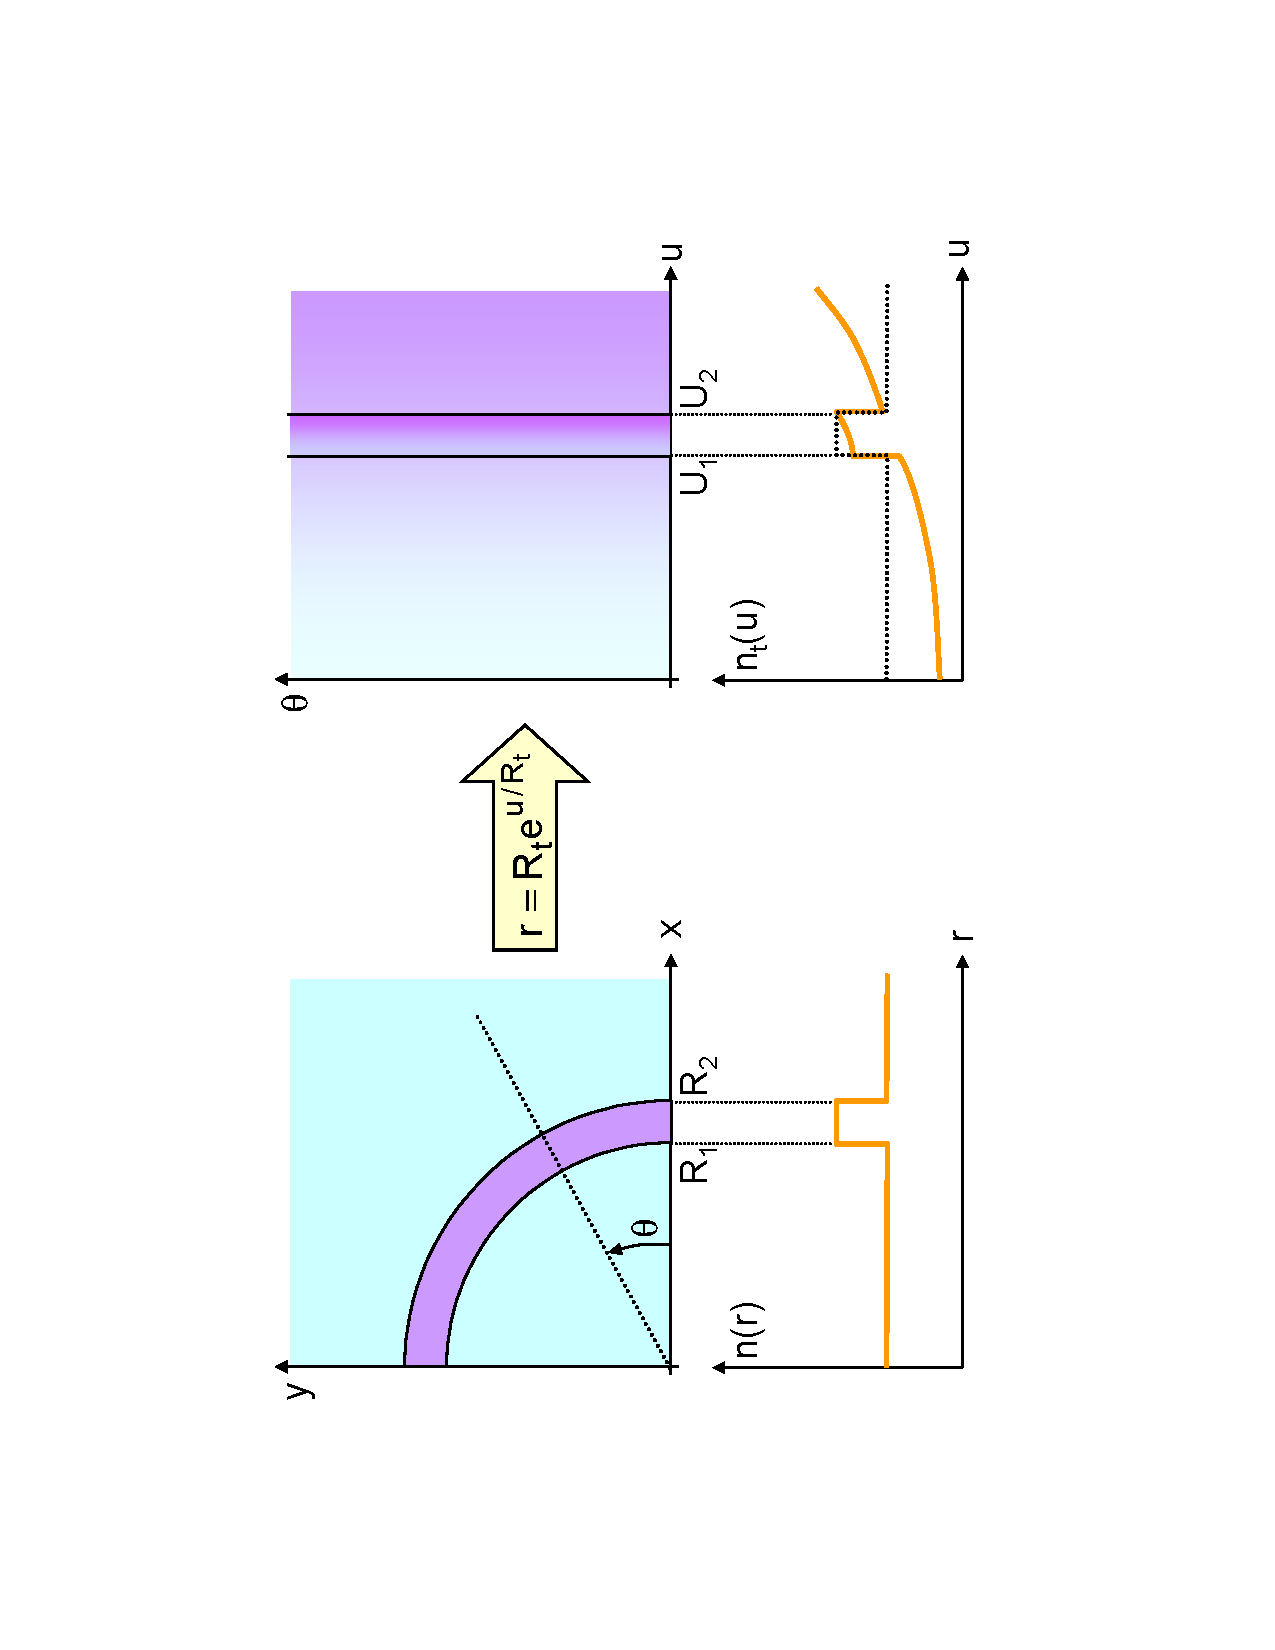
\includegraphics[width=14cm, angle=270]{complex/figures/bends}
\caption{Calculating bend modes using conformal transformation.}
\label{fig-bends}
\end{figure}

To tackle this problem, we could formulate the Helmholtz equation in cylindrical
coordinates, and the solution would involve Bessel functions which we will
introduce in the next chapter. Here however, we will use the following conformal
transformation to convert the curved geometry to a straight one:

\begin{equation}
w = R_t \ln \frac{z}{R_t}
\end{equation} 

$R_t$ is an arbitrary (real) scaling parameter. With $z=r e^{j \theta}$, we can
write this as

\begin{equation}
u + jv = R_t \ln \frac{r}{R_t} + j R_t \theta
\end{equation} 

This clearly shows the effect of the transformation: a circular path in the
$z$--plane with constant $r$ is transformed to a straight path in the $w$--plane
with constant $u$ (see Fig.~\ref{fig-bends}).

Let's now calculate the transformation factor $T$ as defined in
Eq.~\ref{eq-T-factor}.

\begin{equation}
\frac{\partial u}{\partial x} = \frac{R_t}{r}\frac{\partial r}{\partial x} = 
\frac{R_t}{\sqrt{x^2+y^2}} \cdot \frac{2x}{2\sqrt{x^2+y^2}} = R_t
\frac{x}{x^2+y^2}
\end{equation} 

Also,

\begin{equation}
\frac{\partial v}{\partial x} = R_t \frac{\partial}{\partial x} \arctan
\frac{y}{x} = \frac{R_t}{1 + \frac{y^2}{x^2}} \cdot y \cdot \frac{-1}{x^2}= -R_t
\frac{y}{x^2+y^2}
\end{equation} 

So finally

\begin{equation}
T = \frac{1}{\sqrt{u_x^2+v_x^2}} = \frac{\sqrt{x^2+y^2}}{R_t} =
\frac{r}{R_t}=e^{\frac{u}{R_t}}
\end{equation} 

In the new coordinate system, the transformed index profile looks like

\begin{equation}
n_t(u) = n(u)e^{\frac{u}{R_t}}
\end{equation} 

This profile is sketched in Fig.~\ref{fig-bends}. The rest of the solution now
proceeds as follows. The continuous index profile is approximated by a stepwise
constant profile with a large number of steps. The modes of such a waveguide can
be readily found by using standard techniques (see e.g. the course
'Microphotonics').

Even without calculating the modes of the transformed waveguide explicitly, we
can gain qualitative insight in their behaviour by looking at the new index
profile. Because the refractive index  is higher near the outside of the bend,
the mode will tend to be concentrated there. For very short bend radii, the mode
will leak towards the outer cladding, where the index is even higher. This is
the origin of the radiation loss in waveguide bends.

\pagebreak
\section*{Augustin Cauchy (1789--1857)}

\parpic{\includegraphics[scale=0.5]{complex/figures/cauchy}}
Augustin Cauchy was the mathematician that set the foundation of rigour in
modern analysis. A product of the revolutions in France during the eighteenth
and nineteenth centuries, he provided the revolutionary ideas that set this
branch of mathematics on its present course. He is also known as being one of
the most prolific writers in the history of the science.

Augustin Louis Cauchy was born in Paris, France, on August 21, 1789, only a
month after the storming of the Bastille. His father, a government official and
staunch royalist, recognised the coming revolution and quickly moved his family
to a country cottage in Arcueil. Having escaped the guillotine, the family was
poor and the young boy was generally malnourished. For the rest of his life,
this early poverty left the future mathematician in a state of ill--health.
During his eleven year stay at the cottage, Augustin received a classical
education and a strong disposition for the monarchy from his father, who wrote
his own textbooks in verse, and strict Catholic religious training from his
mother. This training would influence the rest of his life. His zealous
political and religious beliefs would alienate this great mathematician from the
majority of his countrymen.


In 1800, the Cauchy's family returned to Paris after the political situation
stabilised. During this early period in his life, Augustin's talent was
recognised by two great mathematicians, Marquis Laplace and Joseph Lagrange.
Both, after seeing the young boy's work, encouraged him to continue in
mathematics. As Lagrange once predicted, he would eventually outdo both of them.
Cauchy's education, however, was in engineering. After attending the Ecole
Polytechnique, a military engineering school taught by some of the country's
greatest mathematicians, and the Ecole des Ponts et Chaussees, he took a
position as an engineer in Napoleon's army at Cherbourg. Somehow during his busy
schedule, he found time to dabble in mathematics. During his three years there,
he produced several significant mathematical papers, including one on
determinants that gave the term its modern meaning. All this mathematical output
also accomplished to ruin his health and ended his career in military
engineering.


Now with all his efforts focused on mathematics, Cauchy became a star on the
mathematics scene. After a slew of achievements, he became a professor at the
Polytechnique in 1816. Then at the unheard of age of 27, he was elected to the
Academy of Sciences in Paris. To be selected for the Academy was one of the
highest honours that could be given to a scientist. Unfortunately, his
acceptance of the position was filled with controversy. At the time, Napoleon
had just been overthrown and the Bourbons had been returned to the throne. The
new king immediately went about removing the former emperor's supporters
including Gaspard Monge, a member of the Academy. Despite his political views,
Monge was one of the greatest mathematicians in France and his removal was
considered an outrage. However, when Cauchy was offered his seat, he accepted
without reserve. Being a staunch royalist, he saw nothing wrong with the removal
of an enemy of the king and saw it as his duty to the monarchy to take the
position. This action did not bode well with many of countrymen and made him
many enemies. Nevertheless, the mathematician continued his work and somehow
found time to be married two years later.


This would not be the last time his political views would get him into trouble.
In 1830 after the overthrow of King Charles X, all members of the Academy were
obligated to swear an oath of allegiance to the new king. Having already taken
an oath to Charles, Cauchy refused. He was removed from his position and
self--exiled to Switzerland without his family. There he became a professor at
the University of Turin and planned to spend the rest of his life working on
mathematics. That was not to be. Two years later, Charles X, now in exile, asked
the professor to supervise the education of his heir Henri. Being a good
royalist, he agreed and was joined with his family in Vienna. His new duties
overwhelmed him and his mathematical work lessened to a trickle. He found his
escape in 1838 when he returned to Paris. Before he left, the king had given him
the impressive sounding but practically useless title of baron. He still refused
to take the oath and constantly struggled to find and hold a position. Finally
in 1848, the oath was abolished and he resumed his old posts. Recognising his
value to Academy, he was exempted when the oath was reestablished in 1852.


Augustin Cauchy died on May 23, 1857, after contracting a fever on a trip to the
country to help restore his health. His last words were, "Men die but their
works endure."


Cauchy's life was one as unusual and complicated as the times he lived in.
Brought up as a devout Catholic in a time most Frenchmen were opposed to the
Church, he suffered prejudice from many people. However, the discrimination did
not discourage him from engaging in his life's favourite hobby, charity. When he
was not involved in some math problem, he was often working on some new mercy
mission for the less fortunate. On the other hand, he could be bigoted against
those who did not hold his religious views. For example, part of the reason
Cauchy delayed the publication of fellow mathematician Niels Abel's masterpiece
was because the latter called him a "bigoted Catholic."


He also tended to be just as opinionated in matters of politics. A supporter of
the monarchy, he came into direct conflict with the supporters of both the
republic and Napoleon. Again, he was both discriminated against and prejudiced
against others. On one hand, his life was put into constant turmoil because of
the affair with the oath. On the other hand, he helped repress the mathematical
work of Nicolas Galois because the latter was a radical republican. Certainly,
Cauchy led a very complicated and intricate life.


Cauchy is famous in the field of mathematics for two main reasons: his numerous
contributions to the science and his immense publishing. His works spanned every
branch of mathematics and are simply too long to list. He is especially famous
for his works with convergent series and rigour in analysis. Early in his
career, Cauchy developed the criteria for determining if an infinite series is
convergent or divergent. While attending a lecture on the subject, it is told
that Laplace became panicked and rushed home. He had just finished his
masterpiece that used infinite series as its backbone and desperately checked
each one for convergence, which they did. Cauchy second great contribution was
setting the groundwork for rigour in analysis and all of mathematics. Rigour is
discovery of the logical foundations of a science. Over the previous centuries,
mathematicians had tried in vain to discover what were the underlying principles
of calculus and many had asserted that Newton's discovery was flawed. Cauchy
took the first step toward unifying the science. First, he defined continuity
and derivative in terms of the limit. Second, he gave the first good definition
of the limit as : "When the values successively assigned to the same variable
indefinitely approach a fixed value, so as to end by differing from it as little
as desired, this fixed value is called the limit of all the others." Though this
is not a mathematical definition, it is a good approximation of the idea, which
would be further clarified by future mathematicians. Other important works
include determinants, polygonal numbers, complex numbers and the theory of
substitutions.


Cauchy is also famous for his writings. Simply put, he overwhelmed the
mathematics world with the number and size of his works. All in all, his total
output included 789 full length papers, one of the largest outputs ever. It was
not uncommon for him to finish two such papers in one week. In addition, these
works tended to be rather long, sometimes extending for over 300 pages. In fact,
after submitting several large papers to be published in the weekly bulletin,
the Academy was forced to limit submissions to four pages to save their small
budget from Cauchy's pen. However, all this writing did get his work out into
the public and spread his ideas. A lot of his fame can be assessed to the fact
that he simply overwhelmed all his competitors on the bookshelves. Because of
this fact, his name is prominent in almost any analysis textbook.

(Paul Golba, from http://www.shu.edu/projects/reals/history/cauchy.html)
